\documentclass{standalone}
\usepackage{tikz}

\usetikzlibrary{arrows, positioning}

\tikzset{
    stage/.style = { draw, thick, 
        rectangle, align=center,
        rounded corners=2mm
    },
    arrow/.style = { -latex, very thick }
}

\begin{document}
    \begin{tikzpicture}
        \node[stage] (0) at (0,0) {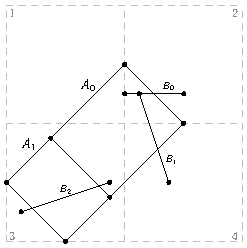
\includegraphics[]{DAC1}};
        \node[scale=1.5] (A) [below = 2mm of 0] {(a)};
        
        \node[stage] (1) [right = 10mm of 0] {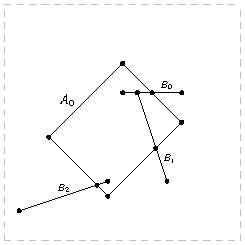
\includegraphics[]{DAC2}};
        \node[scale=1.5] (B) [below = 2mm of 1] {(b)};
        
        \node[stage] (2) [right = 10mm of 1] {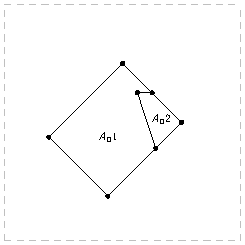
\includegraphics[]{DAC3}};
        \node[scale=1.5] (C) [below = 2mm of 2] {(c)};
        
        \draw[arrow] (0) --  (1);
        \draw[arrow] (1) --  (2);
    \end{tikzpicture}
\end{document}
